O HSM é composto de duas estruturas com saliências, o rotor e o estator, seu circuito magnético é excitado pela combinação de espiras e magnetismo permanente, imã. As espiras são montadas nos polos do estator e o imã no rotor. Tipicamento o motor de passo híbrido tem oito polos no estator e em cada polo tem entre dois a seis dentes, ou também chamado \emph{teeth}, do inglês. Comumente ele tem uma pequena largura de passo, tipicamente 1,8º. 

A Fig. \ref{fig:estrutura_HSM} ilustra um HSM típico, onde é colocado um íma no centro das duas partes constituintes do rotor de forma a magnetizá-lo com as duas polaridades, pois seria excessivamente caro confeccionar o rotor inteiramente como um bloco de imã. A seção X é mostrada como um corte frontal do motor logo abaixo, bem como a seção Y é um corte do ponto de vista do fundo de quem olha o motor. Os enrolamentos são colocados em volta das seções do estator, de forma que um enrolamento abranja uma certa quantidade de dentes. \cite{SteppingBook}

\begin{figure}[H]
	\centering
	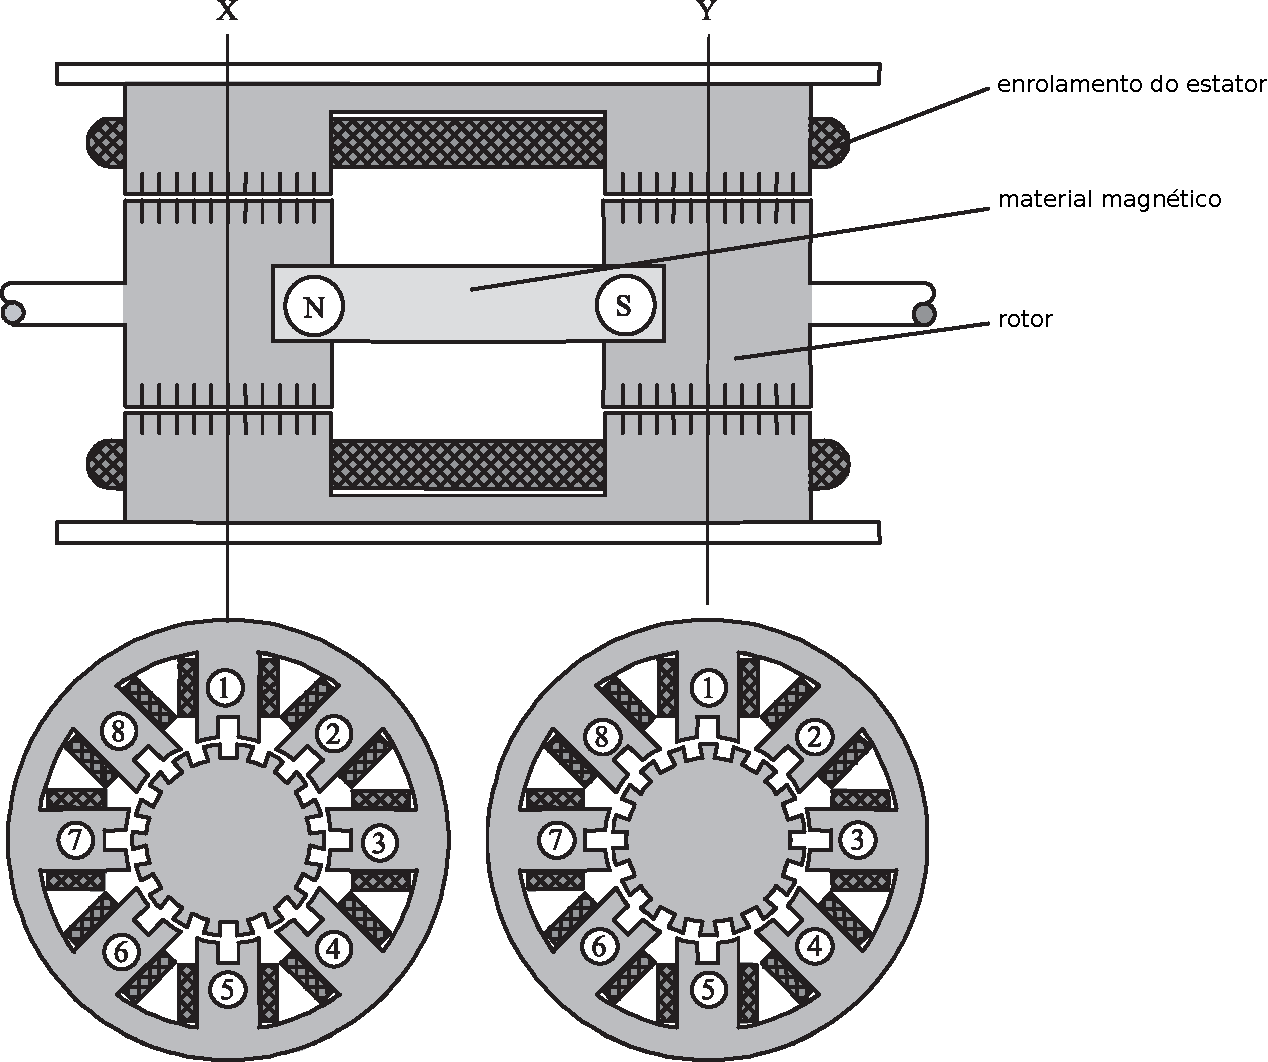
\includegraphics[width = \columnwidth]{Images/estrutura_HSM.pdf}
	\caption{Visão de lado, frente e costas do HSM. \cite{SteppingBook}}
	\label{fig:estrutura_HSM}
\end{figure}

O rotor é construído de tal forma que os dentes do polo sul fiquem alinhados entre dois dentes do polo norte, ou vise versa, mais claramente percebível na Fig. \ref{fig:HSM_dentes}, esta compensação é chamada de \textit{offset} como citado anteriormente. Isto é feito para que haja o troque no eixo devido a força magnética de atração de polos diferentes e repulsão de iguais, pois se os dentes da parte sul estivessem alinhados aos da face norte não haveria este torque, pois estaria para um dado dente do estator um polo norte e sul, se cancelando as forças de atração e repulsão.

\begin{figure}[!h]
	\centering
	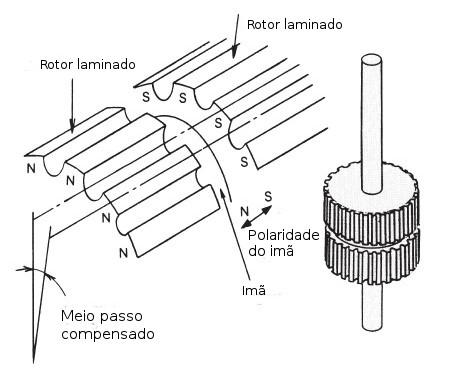
\includegraphics[width = \columnwidth]{Images/VR_ROTOR.jpg}
	\caption{Detalhe de construção do rotor do HSM. \cite{angulo_rotor}}
	\label{fig:HSM_dentes}
\end{figure}

As principais partes constituintes de um HSM comercial é mostrado na Fig. \ref{fig:partes_SM}. Pela figura é possível identificar que o imã é um disco que fica entre a parte do sul e norte do rotor, de tal forma que a polaridade do imã permeie pelo material magnético laminado do rotor. Tanto o rotor e o estator são materiais magnéticos laminados, a laminação é para reduzir a formação de correntes parasitas que diminuem a eficiência da máquina.

\begin{figure*}[!t]
	\centering
	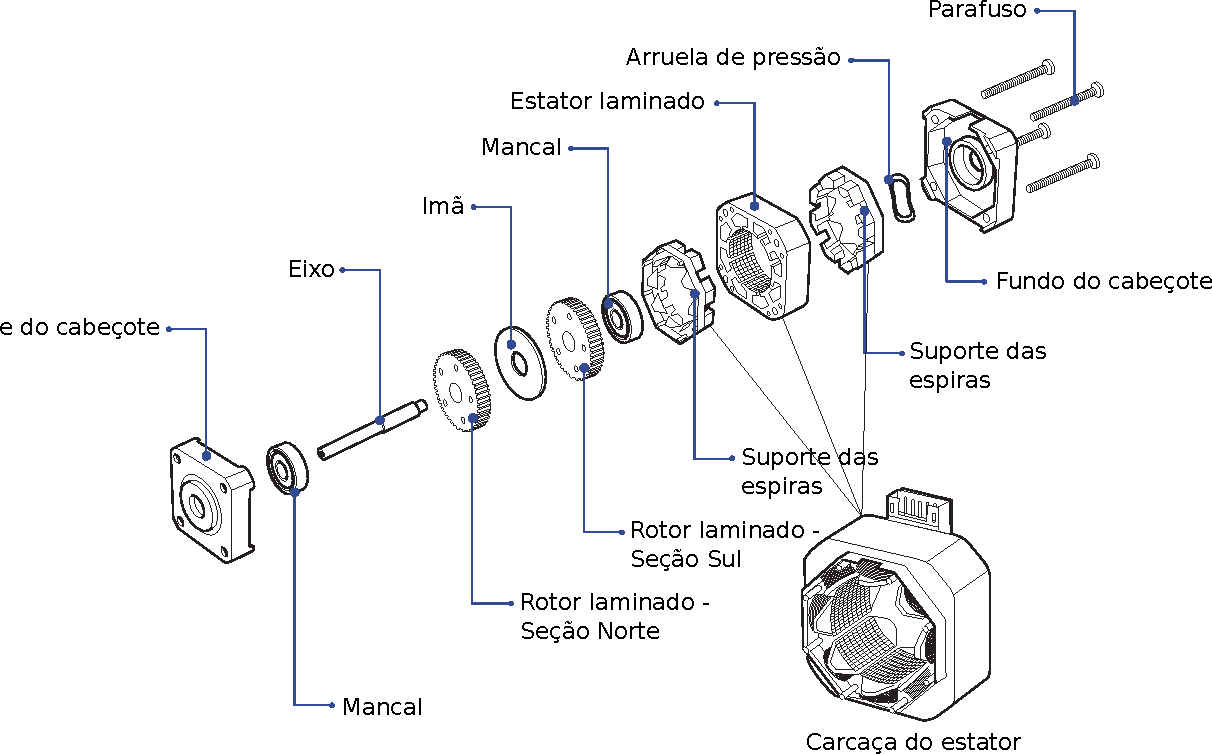
\includegraphics[width = .8\textwidth]{Images/partes_HSM.pdf}
	\caption{Partes constituintes de um HSM comercial. \cite{MoonsHSM}}
	\label{fig:partes_SM}
\end{figure*}
